\section{Cohomology}
\subsection{de Rham complex}

    \newdef{Exact form}{\index{exact}
        If $\omega\in\Omega^k(M)$ can be written as $\omega = d\chi$ for some $\chi\in\Omega^{k-1}(M)$, it is said to be exact. We can conclude that
        \begin{gather}
            \text{im}(d_k) = \{\omega\in\Omega^{k+1}(M):\omega\text{ is exact}\}.
        \end{gather}
    }
    \newdef{Closed form}{\index{closed}
        Let $\omega\in\Omega^k(M)$. If $d\omega = 0$, it is said to be closed. We can conclude that
        \begin{gather}
            \{\omega\in\Omega^k(M):\omega\text{ is closed}\}\subseteq\text{ker}(d_k).
        \end{gather}
    }

    \begin{remark}\label{diff:closed_exact}
        From the first item of property \ref{diff:exterior_derivative_properties} it follows that every exact form is closed. The converse, however, is not true\footnote{See result \ref{diff:poincare} below for more information.}.
    \end{remark}

    \newdef{de Rham complex}{
        The sequence
        \begin{gather}
            0\longrightarrow\Omega^0(M)\longrightarrow\Omega^1(M)\longrightarrow\cdots\longrightarrow\Omega^{\dim(M)}(M)\longrightarrow0
        \end{gather}
        together with the sequence of exterior derivatives $d_k$ forms a cochain complex by property \ref{diff:exterior_derivative_properties}. This complex is called the de Rham complex $H^\bullet_{dR}(M)$.
    }

    The relation between closed and exact forms can be used to define the de Rham cohomology groups:
    \newdef{de Rham cohomology}{\index{de Rham!cohomology|see{cohomology}}\index{cohomology!de Rham}\label{diff:de_rham_cohomology}
        Following definition \ref{homalg:homology} we define the $k^{th}$ de Rham cohomology group on $M$ as the following quotient space:
        \begin{gather}
            H^k_{dR}(M) := \frac{\text{ker}(d_k)}{\text{im}(d_{k-1})}.
        \end{gather}
        This quotient space is a vector space. Two elements of the same equivalence class in $H^k_{dR}(M)$ are said to be \textbf{cohomologous}.
    }

    \newdef{Integral form}{\label{diff:integral_form}\index{integral!form}
        A closed $k$-form $\omega$ is said to be integral if it lies in the image of the inclusion $H^k(M, \mathbb{Z})\hookrightarrow H^k(M, \mathbb{R})$. Equivalently, a closed $k$-form is integral if integrating it over any $k$-cycle with integral coefficients gives an integer.
    }

    \newformula{Cup product}{\index{cup product}\label{diff:cup_product}
        Let $[\nu]\in H^k_{dR}$ and $[\omega]\in H^l_{dR}$. The cup product on de Rham cohomology is given by
        \begin{gather}
            [\nu]\smile[\omega] := [\nu\wedge\omega].
        \end{gather}
    }

    The following theorem allows us to write $H^\bullet(M)$ for the de Rham cohomology on $M$:
    \begin{theorem}[de Rham]\index{de Rham}
        The de Rham cohomology over a smooth manifold $M$ is isomorphic to the singular cohomology\footnote{See section \ref{section:singular_homology} for more information.} over $M$.
    \end{theorem}

    \begin{theorem}[Poincar\'e lemma\footnotemark]\index{Poincar\'e}\label{diff:poincare}
        \footnotetext{The original theorem states that on a contractible space (see definition \ref{topology:contractible_space}) every closed form is exact.}
         For every point $p\in M$ there exists a neighbourhood on which the de Rham cohomology is trivial:
        \begin{gather}
            \forall p\in M:\exists U\subseteq M: H^k(U) = 0.
        \end{gather}
        This implies that every closed form is locally exact, i.e. if $d\omega=0$ at the point $p\in M$ then there exist a neighbourhood $U\subseteq M$ of $p$ and a differential form $\lambda$ such that
        \begin{gather}
            \omega = d\lambda
        \end{gather}
        at all points $p'\in U$. More generally, this lemma says that the following isomorphism exists for every smooth manifold $M$:
        \begin{gather}
            H^\bullet(M\times\mathbb{R}^n) \cong H^\bullet(M).
        \end{gather}
        In fact, this can even be further generalized due to the homotopy axiom of de Rham cohomology:
        \begin{gather}
            H^\bullet(E) \cong H^\bullet(M)
        \end{gather}
        for every vector bundle $E$ over $M$.
    \end{theorem}

    \newdef{Relative cohomology}{
        Consider the submanifold inclusion $\iota:S\hookrightarrow M$. The relative de Rham complex is defined as follows:
        \begin{gather}
            \Omega^n(M, S) := \Omega^n(M)\oplus\Omega^{n-1}(S)
        \end{gather}
        where the coboundary operator $d$ is defined by $d(\omega,\lambda) := (d\omega, \iota^*\omega-d\lambda)$. The relative de Rham cohomology $H^\bullet(M, S)$ is defined as the cohomology of this complex. Classes are represented by closed forms on $M$ that restrict to exact forms on $S$.

        This definition can in fact be generalized to any smooth map $f:M\rightarrow N$ by replacing $\iota^*$ in the coboundary by $f^*$. This cohomology ring is denoted by $H^\bullet(f)$. For all smooth maps $f$ we obtain the following long exact sequence:
        \begin{gather}
            \cdots\longrightarrow H^k(f)\longrightarrow H^k(M)\longrightarrow H^k(N)\longrightarrow H^{k+1}(f)\longrightarrow\cdots.
        \end{gather}
    }

\subsection{Integration}\index{co-!chain}

    Now, we can also give a little side note about why the de Rham cohomology groups \ref{diff:de_rham_cohomology} really form a cohomology theory. For this we need some concepts from homology which can be found in section \ref{section:homology}. Let $M$ be a compact differentiable manifold and let $\{\lambda_i:\Delta^k\rightarrow M\}$ be the set of singular $k$-simplexes on $M$.

    Suppose that we want to integrate a form over a singular $k$-chain $C = \sum_{i=0}^ka_i\lambda_i$ on $M$. By integration we can pair the $k$-form $\omega$ and the chain $C$ as if they are dual objects (hence $p$-forms are also called $p$-\textbf{cochains}) to produce a real number\footnote{This requires the chain group to have real coefficients instead of integer coefficients as is mostly used in homology.}:
    \begin{gather}
        \langle\cdot,C\rangle:\Omega^n(M)\rightarrow\mathbb{R}:\omega\mapsto\int_C\omega = \sum_{i=0}^ka_i\int_{\Delta_k}\lambda_i^{*}\omega
    \end{gather}
    where $\lambda_i^*$ pulls $\omega$ back to $\Delta^k$ (which is a subset of $\mathbb{R}^k$ as required). Stokes's theorem \ref{diff:stokes_theorem} then tells us that
    \begin{gather}
        \int_Cd\omega = \int_{\partial C}\omega.
    \end{gather}
    Using the pairing $\langle\cdot,\cdot\rangle$ this can be rewritten more explicitly as
    \begin{gather}
        \langle d\omega, C\rangle = \langle \omega, \partial C\rangle.
    \end{gather}
    The operators $d$ and $\partial$ can thus be interpreted as formal adjoints. After checking (again using Stokes' theorem) that all chains $C$ and cochains $\omega$ belonging to the same equivalence classes $[C]\in H_k(M; \mathbb{R})$ and $[\omega]\in H^k(M; \mathbb{R})$ give rise to the same number $\langle\omega, C\rangle$, we see that the singular homology groups and the de Rham cohomology groups on $M$ are well-defined dual groups. The name \textit{co}homology is thus well-chosen for \ref{diff:de_rham_cohomology}.

\subsection{Cohomology with compact support}\index{cohomology!compact support}

    Because of integration is involved in all statements in this section, we will assume all manifolds and bundles to be orientable unless states otherwise.

    The following definition characterizes cohomology with compact support directly through its relation to compact sets:
    \newadef{Cohomology with compact support}{
        Consider a (not necessarily orientable) manifold $M$. The cohomology with compact support $H^\bullet_c(M)$ can be defined as the following direct limit:
        \begin{gather}
            H^\bullet_c(M) := \varinjlim_{K\text{ compact}}H^\bullet(M, M\backslash K).
        \end{gather}
    }
    \begin{property}[Relation to reduced cohomology]\label{diff:reduced_compact_cohomology}
        For any topological space $X$, the inclusion $U\hookrightarrow X$ for any open $U$ induces a long exact sequence in compactly supported cohomology. Performing excision by $V:=X\backslash U$ in the above definition of compact cohomology gives $H(X, X\backslash K \cup V)\cong H^\bullet(U, U\backslash K)$ and thus $H^\bullet_c(X, V)\cong H^\bullet_c(U)$. The long exact sequence for compact cohomology can therefore be rewritten in terms of the compactly supported cohomologies of $U,V$ and $X$.

        If we choose $X$ to be the one-point compactification $\widehat{M}$ of $M$ and take $U=M$, then the aforementioned long exact sequence implies that
        \begin{gather}
            H^\bullet_c(M)\cong H^\bullet(\widehat{M}, \ast)\cong\widetilde{H}^\bullet(\widehat{M})
        \end{gather}
        where we used that both $\ast$ and $\widehat{M}$ are compact.\footnote{This is true for Hausdorff spaces.}
    \end{property}

    \begin{theorem}[Poincar\'e duality]\index{Poincar\'e!duality}\label{diff:poincare_duality}
        Let $M$ be a smooth $m$-dimensional manifold. The pairing $\int:H^k(M)\otimes H^{m-k}_c(M)\rightarrow\mathbb{R}$ induces an isomorphism on cohomology:
        \begin{gather}
            H^k(M)\cong\Big(H^{m-k}_c(M)\Big)^*.
        \end{gather}
        If $M$ is of finite type the converse also holds
        \begin{gather}
            H^k_c(M)\cong\Big(H^{m-k}(M)\Big)^*.
        \end{gather}
    \end{theorem}
    \begin{result}[Poincar\'e lemma for compact cohomology]\index{Poincar\'e!lemma}
        Let $M$ be a (not necessarily orientable) smooth manifold of finite type. For every rank-$n$ vector bundle $E$ over $M$ the following isomorphism exists
        \begin{gather}
            H^\bullet_c(E)\cong H^{\bullet-n}_c(M).
        \end{gather}
    \end{result}

    \newdef{Poincar\'e dual}{\index{dual!Poincar\'e|see{Poincar\'e duality}}
        Let $M$ be a smooth $m$-dimensional manifold and let $i:S\rightarrow M$ be a closed $k$-dimensional submanifold. The Poincar\'e dual of $S$ in $M$ is the unique cohomology class $[\eta_S]\in H^{m-k}(M)$ such that
        \begin{gather}
            \int_Si^*\omega = \int_M\omega\wedge\eta_S
        \end{gather}
        for all compactly supported $\omega\in H^k_c(M)$.

        If $S$ is compact in $M$, two Poincar\'e duals exist:
        \begin{itemize}
            \item \textbf{Closed dual}: The Poincar\'e dual obtained by using the fact that $S$ is compact and hence closed in $M$.
            \item \textbf{Compact dual}: Because $S$ is compact, all forms $\omega\in H^k(M)$ (not only the compactly supported ones) can be integrated over $S$ and, assuming $M$ is of finite type, Poincar\'e duality implies that there exists a unique cohomology class with compact support $\eta_S'$ such that
            \begin{gather}
                \int_Si^*\omega = \int_M\omega\wedge\eta'_S
            \end{gather}
            for all $\omega\in H^k(M)$.
        \end{itemize}
    }
    \remark{Because the compact Poincar\'e dual induces a pairing on all closed forms $\omega$, which include the compactly supported ones, the compact dual is (as a form) equal to the closed Poincar\'e dual. However, as elements in cohomology these can be quite different.}

    \begin{property}[Localization principle]\index{localization}
        The support of the compact Poincar\'e dual of a compact submanifold $S$ may be shrunk to any neighbourhood of $S$. More generally, the support of the (closed) Poincar\'e dual of a closed submanifold $S$ can be shrunk to any tubular neighbourhood of $S$.
    \end{property}

    \begin{formula}[Transversal intersections]
        The Poincar\'e dual of a transversal intersection is equal to the wedge product of the individual Poincar\'e duals:
        \begin{gather}
            \eta_{S\cap T} = \eta_S\wedge\eta_T.
        \end{gather}
    \end{formula}

    \begin{definition}\index{cohomology!vertical support}
        Let $\pi:E\rightarrow M$ be a smooth vector bundle over $M$. A differential form $\omega\in\Omega^\bullet(E)$ is an element of $\Omega^\bullet_{cv}(E)$ if $\text{supp}(\omega)\cap\pi^{-1}(K)$ is compact for every compact subset $K\subset M$. The cohomology of this complex is called the \textbf{de Rham cohomology with compact support in the vertical direction} or \textbf{compact vertical cohomology}.
    \end{definition}
    \begin{remark}
        The above definition implies that $\omega\in\Omega^\bullet_{cv}(E)$ is compactly supported on each fibre $\pi^{-1}(p),p\in M$. This observation explains the name of the cohomology theory.
    \end{remark}

    \newdef{Fibre integration}{\index{fibre!intregation}
        Differential forms with vertically compact support on a rank-$n$ vector bundle $\pi:E\rightarrow M$ can be divided into two classes:
        \begin{itemize}
            \item \textbf{Type 1}: those locally of the form $f(x, t)\pi^*\phi\wedge(dt_{i_1}\wedge\cdots\wedge dt_{i_k})$ where $\phi$ is a form on the base manifold $M$, $f$ has compact support and $k<n$.
            \item \textbf{Type 2}: those locally of the form $f(x, t)\pi^*\phi\wedge(dt_1\wedge\cdots\wedge dt_n)$ where $\phi$ is a form on the base manifold $M$ and $f$ has compact support.
        \end{itemize}
        We define the fibre integration map $\pi_*:\Omega^\bullet_{cv}(E)\rightarrow\Omega^{\bullet-n}(M)$ as follows: If $\omega$ is of type 1, then $\pi_*\omega := 0$. If $\omega$ is of type 2, then
        \begin{gather}
            \pi_*\omega := \left(\idotsint f(x, t)dt_1\cdots dt_n\right)\phi.
        \end{gather}
    }

    \begin{formula}[Projection formula]\index{projection!formula}
        Consider a rank-$n$ vector bundle $\pi:E\rightarrow M$. For every pair of forms $\phi\in\Omega^\bullet(M)$ and $\omega\in\Omega^\bullet_{cv}(E)$ the following formula holds:
        \begin{gather}
            \pi_*(\pi^*\phi\wedge\omega) = \phi\wedge\pi_*\omega.
        \end{gather}
        Furthermore, if $\phi\in\Omega^k_c(M)$ and $\omega\in\Omega^{m+n-k}_{cv}(E)$, then
        \begin{gather}
            \int_E\pi^*\phi\wedge\omega = \int_M\phi\wedge\pi_*\omega.
        \end{gather}
    \end{formula}

    \begin{theorem}[Thom isomorphism]\index{Thom!isomorphism}
        For every rank-$n$ vector bundle $\pi:E\rightarrow M$, where $M$ is (not necessarily orientable and) of finite type, fibre integration gives the following isomorphism:
        \begin{gather}
            \pi_*:H^\bullet_{cv}(E)\cong H^{\bullet-n}(M):\mathcal{T}.
        \end{gather}
    \end{theorem}
    \begin{result}[Poincar\'e lemma for vertically compact cohomology]\index{Poincar\'e!lemma}
        \begin{gather}
            H^\bullet_{cv}(M\times\mathbb{R}^n)\cong H^{\bullet-n}(M).
        \end{gather}
    \end{result}

    \newdef{Thom class}{\index{Thom!class}
        The image $\Phi$ of $1\in H^0(M)$ under the Thom isomorphism.
    }
    \begin{formula}[Thom isomorphism]
        Because $\mathcal{T}$ and $\pi_*$ are inverses, and hence $\pi_*\Phi = 1$, the projection formula implies that
        \begin{gather}
            \mathcal{T}(\omega) = \pi^*\omega\wedge\Phi.
        \end{gather}
    \end{formula}

    \begin{property}[Orientation class]
        The Thom class $\Phi$ restricts to a generator of \[H^n_c(F)\cong \widetilde{H}^n(S^n)\cong H^n(S^n).\] For compact orientable manifolds (such as $S^n$) such a generator gives rise to a generator of the homology group $H_n$, i.e. it gives rise to an orientation class \ref{diff:orientation_class}.
    \end{property}
    \begin{property}[Poincar\'e dual through Thom class]\index{Poincar\'e!dual}
        The Poincar\'e dual of a closed submanifold is equal to the Thom class of its normal bundle.
    \end{property}

    We now elaborate a bit more on the technicalities of the Thom isomorphism. For example, the fact that throughout the literature the Thom isomorphism is stated in various forms using compactly supported cohomology, relative cohomology and reduced cohomology.

    \newdef{Thom space}{\index{Thom!space}\index{sphere!bundle}
        Let $E\rightarrow M$ be a vector bundle. For every fibre in $E$ we can construct its one-point compactification \ref{topology:alexandrov_compactification} and by gluing these together we obtain the \textbf{sphere bundle} $\text{Sph}(E)$. The quotient space $\text{Sph}(E)/B$, where we identify all the adjoined points, is called the Thom space $\text{Th}(E)$.

        If we are handed a metric on $E$ (see chapter \ref{chapter:riemann}) we can give an alternative definition: Let $V$ be the typical fibre of $E$. We can construct a new bundle, the unit sphere bundle $S(E)$, where the typical fibre is the unit sphere $S(V) := \{v\in V : ||v|| = 1\}$. It should be noted that this new bundle is not a vector bundle since the unit sphere is not a vector space. A similar construction leads to the unit disk bundle $D(E)$ where the typical fibre is the unit disk $D(V) := \{v\in V : ||v||\leq1\}$. The Thom space $\text{Th}(E)$ can be shown to be isomorphic to the quotient space $S(E)/D(E)$.
    }
    \begin{property}
        If the base manifold $M$ is compact, the Thom space is obtained as the one-point compactification of the total space $E$.
    \end{property}

    \begin{property}[Different forms of Thom isomorphism]
        Let $E\rightarrow M$ be a vector bundle. We denote the complement of the zero section by $E_0$ as in \ref{diff:zero_section}. Homotopy invariance implies that
        \begin{gather}
            H^\bullet(D(E), S(E))\cong H^\bullet(E, E_0).
        \end{gather}
        Then, using result \ref{diff:ndr_submanifold} together with the dual of property \ref{topology:ndr_pair_homology}, we can show that the reduced cohomology of the Thom space $\text{Th}(E)$ is isomorphic to the relative cohomology of the pair $(E, E_0)$:
        \begin{gather}
            \widetilde{H}^\bullet(\text{Th}(E))\cong H^\bullet(E, E_0).
        \end{gather}
        To relate this to vertically compact cohomology we slightly adapt property \ref{diff:reduced_compact_cohomology}. Compact support gave rise to the (reduced) cohomology of the compactified space. By analogy we expect that vertically compact support should correspond to compactifications of the fibres. However, this is exactly how the Thom space was constructed.

        The above arguments finally lead to the following ''triangle'' of isomorphisms:
        \begin{gather}
            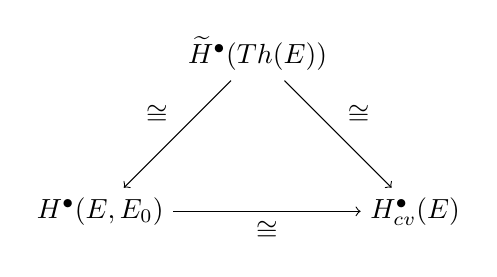
\begin{tikzpicture}[baseline=(current bounding box.east)]
                \node (TH) at (0, 0) {$\widetilde{H}^\bullet(\text{Th}(E))$};
                \node (R) at (-2, -2) {$H^\bullet(E, E_0)$};
                \node (CV) at (2, -2) {$H^\bullet_{cv}(E)$};
                \draw[->] (TH) -- node[above left]{$\cong$} (R);
                \draw[->] (TH) -- node[above right]{$\cong$} (CV);
                \draw[->] (R) -- node[below]{$\cong$} (CV);
            \end{tikzpicture}
        \end{gather}
    \end{property}

    \newdef{Thom spectrum}{\index{spectrum!Thom}
        Let $E\rightarrow M$ be a vector bundle. The Thom spectrum of $E$ is defined as the suspension spectrum of its Thom space. This can be written more explicitly as
        \begin{gather}
            (\Sigma^\infty\text{Th}(E))_n\cong\text{Th}(\mathbb{R}^n\oplus E)
        \end{gather}
        because of the existence of a homeomorphism $\text{Th}(\mathbb{R}^n\oplus E)\cong\Sigma^n\text{Th}(E)$.

        Let us now consider the sequence $\seq{\xi}$ of universal vector bundles. For every $\xi_n$ we define the $n^{th}$ component space as follows:
        \begin{gather}
            MO_n := \text{Th}(\xi_n).
        \end{gather}
        The Whitney sum $\xi_n\oplus\mathbb{R}$ can be obtained as a pullback of $\xi_{n+1}$. This map induces a map $\Sigma MO_n\rightarrow MO_{n+1}$, which gives the $n^{th}$ structure map of ''the'' Thom spectrum $MO$.\footnote{Note that the Thom spectrum as defined here is not an $\Omega$-spectrum \ref{topology:spectrum}, it is merely a sequential spectrum (prespectrum).}
    }

    \newdef{Euler class}{\index{Euler!class}
        Consider a vector bundle $E\rightarrow M$ together with its Thom class $\Phi$. The Euler class $e(E)$ is defined as the pullback $s_0^*\Phi$ of the Thom class along the zero section of $E$.
    }
    \begin{property}
        If the orientation of $E$ is reversed, the Euler class changes sign.
    \end{property}
    The following property distinguishes the Euler class among all characteristic classes of $E$:
    \begin{property}[Normalization]
        If the vector bundle admits a nowhere-vanishing section, its Euler class vanishes.
    \end{property}

\subsection{\v{C}ech-de Rham complex}\label{section:cech_de_rham}

    \begin{theorem}[Mayer-Vietoris sequence]\index{Mayer-Vietoris sequence}
        Consider a smooth manifold $M$ with an open covering $U\cup V$. The cohomology of $U,V$ is related to that of $M$ by the following short exact sequence:
        \begin{gather}
            0\longrightarrow H^\bullet(M)\longrightarrow H^\bullet(U)\oplus H^\bullet(V)\longrightarrow H^\bullet(U\cap V)\longrightarrow 0
        \end{gather}
        where the second arrow acts by restriction and the third one maps $(\omega,\rho)$ to $\rho-\omega$.
    \end{theorem}

    \newdef{\v{C}ech-de Rham complex}{
        Consider an open cover $\mathcal{U}=\{U_i\subseteq M\}_{i\in I}$ of a smooth manifold $M$.\footnote{Some authors require $I$ to be countable.} By $U_{i_0\ldots i_{k-1}}$ we denote the $k$-fold intersection $U_{i_0}\cap\cdots\cap U_{i_{k-1}}$. For all $k$ we define maps (where we suppress the label $k$) \[\delta_j:\Omega^\bullet(U_{i_0\ldots i_{k-1}})\rightarrow\prod_\alpha\Omega^\bullet(U_{i_0\ldots i_{j-1}\alpha i_j\ldots i_{k-1}})\] induced by the inclusions \[\iota_j:U_{i_0\ldots i_k}\hookrightarrow U_{i_0\ldots i_{j-1}i_{j+1}\ldots i_k}\] that ''ignore'' the $j^{th}$ open set. A total coboundary map $\delta$ is then defined as the alternating sum of the $\delta_i$'s:
        \begin{gather}
            (\delta\omega)_{i_0\ldots i_k} = \sum_{j=0}^k(-1)^i\omega_{i_0\ldots\widehat{i_j}\ldots i_k}
        \end{gather}
        for $\omega\in\prod\Omega^\bullet(U_{i_0\ldots i_{k-1}})$. It can be shown that $\delta$ is indeed a coboundary, i.e. $\delta^2=0$. The double complex $C^p(\mathcal{U}; \Omega^q):=\prod\Omega^q(U_{i_0\ldots i_p})$ with total differential $D=\delta+(-1)^pd$, where $d$ is the ordinary de Rham differential, is called the \v{C}ech-de Rham complex.
    }

    The Mayer-Vietoris sequence can be generalized to a statement for the \v{C}ech-de Rham complex:
    \begin{property}[Mayer-Vietoris sequence]
        The horizontal complex
        \begin{gather}
            0\longrightarrow\Omega^\bullet(M)\longrightarrow\prod_{i_0}\Omega^\bullet(U_{i_0})\longrightarrow\prod_{i_0,i_1}\Omega^\bullet(U_{i_0i_1})\longrightarrow\cdots
        \end{gather}
        is acyclic, i.e. the $\delta$-cohomology of the \v{C}ech-de Rham complex vanishes.
    \end{property}

    An important corollary is that one can compute the (de Rham) cohomology of $M$ using the above double complex:
    \begin{theorem}
        The restriction map $\Omega^\bullet(M)\rightarrow C^\bullet(\mathcal{U}; \Omega^\bullet)$ induces an isomorphism in cohomology.
    \end{theorem}
    One can also augment the \v{C}ech-de Rham complex in the other direction by the kernel of the de Rham differential in degree 1. These are the locally constant functions on the intersections $U_{i_0\ldots i_p}$. The cohomology of this augmenting sequence $C^\bullet(\mathcal{U}, \underline{\mathbb{R}})$ is called the \textbf{\v{C}ech cohomology} of $M$.\index{Cech!cohomology} By the same reason as for why the Mayer-Vietoris sequence implied the above theorem, we obtain the following theorem:
    \begin{theorem}[\v{C}ech $=$ de Rham]
        For a smooth manifold $M$, admitting a good cover $\mathcal{U}$, the \v{C}ech cohomology of $\mathcal{U}$ is isomorphic to the de Rham cohomology of $M$:
        \begin{gather}
            H^\bullet(M)\cong\check{H}^\bullet(\mathcal{U}; \underline{\mathbb{R}}).
        \end{gather}
    \end{theorem}
    \begin{result}
        All compact manifolds admit a finite good cover and hence have finite-dimensional de Rham cohomology.
    \end{result}

    We will now construct a generalization of \v{C}ech cohomology. The notation $\underline{\mathbb{R}}$ above should remind us of example \ref{sheaf:constant_sheaf}, i.e. $\underline{\mathbb{R}}$ denotes the sheaf of locally constant functions with values in $\mathbb{R}$. Similarly $\Omega^\bullet$ should be regarded as the sheaf of differential forms.
    \newdef{\v{C}ech cohomology}{\index{Cech!cohomology}
        Let $\mathcal{F}$ be a (pre)sheaf of Abelian groups. For an open cover $\mathcal{U}=\{U_i\subseteq M\}_{i\in I}$ we define the cochain groups
        \begin{gather}
            C^p(\mathcal{U};\mathcal{F}) := \prod_{i_0<\cdots<i_p}\mathcal{F}(U_{i_0\ldots i_p})
        \end{gather}
        for all $p\in\mathbb{N}$ as before. Since the (pre)sheaf takes values in Abelian groups we can define the subtraction of elements and hence the definition of the differential $\delta$ still makes sense:
        \begin{gather}
            \delta := \sum_{i=0}^k(-1)^i\mathcal{F}(\iota_i)
        \end{gather}
        where $\iota_i$ are the inclusion maps as before. The $\delta$-cohomology of the complex $C^\bullet(\mathcal{U}; \mathcal{F})$ is called the \v{C}ech cohomology of $\mathcal{U}$ with values in $\mathcal{F}$.

        By taking the direct limit over the direct system of open covers of a smooth manifold $M$ (the partial ordering is given by refinement of covers) one can define the \v{C}ech cohomology $\check{H}^\bullet(M; \mathcal{F})$ of $M$ with values in $\mathcal{F}$.
    }

    By noting that good covers are \textit{cofinal} in the set of open covers one can obtain the following theorem:
    \begin{theorem}[\v{C}ech $=$ de Rham, bis]
        For a smooth manifold the \v{C}ech cohomology of $M$ with values in $\underline{\mathbb{R}}$ is isomorphic to the de Rham cohomology of $M$:
        \begin{gather}
            H^\bullet(M)\cong\check{H}^\bullet(M;\underline{\mathbb{R}}).
        \end{gather}
    \end{theorem}

    \begin{example}[Zeroth cohomology]
        From the general definition of cohomology groups and the specific form of the coboundary operator we find that \[\omega_{\alpha_0}|_{U_{\alpha_0}\cap U_{\alpha_1}}=\omega_{\alpha_1}|_{U_{\alpha_0}\cap U_{\alpha_1}}\] for all $\alpha_0\neq\alpha_1$ and $\omega\in\check{H}^0(M;\mathcal{F})$. This is exactly the defining relation for the (global) sections of $\mathcal{F}$ and hence we obtain (as usual)
        \begin{gather}
            \check{H}^0(M;\mathcal{F})\cong\mathcal{F}(M).
        \end{gather}
    \end{example}

\subsection{Non-orientable manifolds}

    \newdef{Twisted cohomology}{\index{cohomology!twisted}
        Let $E\rightarrow M$ be a flat vector bundle over $M$. By construction \ref{diff:twisted_differential} we know that the algebra $\Omega^\bullet(M)\otimes E$ can be given the structure of a differential graded algebra \ref{linalgebra:dg_algebra} and hence gives rise to a cohomology theory $H^\bullet(M; E)$. This is called the $E$-twisted de Rham cohomology of $M$.
    }
    \begin{remark}
        By the remark following construction \ref{diff:twisted_differential} we should pay attention to what trivialization was used in the construction of $H^\bullet(M; E)$. It can be shown that two trivializations give rise to the same $E$-twisted cohomology if they admit a common refinement for which the induced sections differ by a locally constant matrix $a\in\text{GL}(n, \mathbb{R})$.
    \end{remark}

    If we take $E=o(M)$ to be the orientation line bundle over $M$, we obtain the (honest) densities of remark \ref{diff:honest_density}. The cohomology of this complex is simply called the \textbf{twisted de Rham cohomology}.
    \begin{property}[Isomorphisms]
        The twisted cohomologies defined by two trivializations induced from atlases on $M$ are isomorphic.\footnote{Although we almost always work with natural trivialization, i.e. where the open subsets of $M$ are obtained from charts on $M$, this is not technically necessary. For these ''exotic'' cases, the isomorphisms not always exist.}
    \end{property}
    \begin{property}[Trivial twisting]
        If $M$ is orientable, its twisted cohomology is isomorphic to its ordinary (de Rham) cohomology. More generally, the $E$-twisted de Rham cohomology is isomorphic to the ordinary de Rham cohomology whenever $E$ is trivial.
    \end{property}

    Poincar\'e duality \ref{diff:poincare_duality} can be translated almost verbatim to the twisted case:
    \begin{theorem}[Poincar\'e duality]\index{Poincar\'e!duality}
        Integration of densities induces the following isomorphism:
        \begin{gather}
            H^k(M)\cong\left(H^{m-k}_c(M; o(M))\right)^*.
        \end{gather}
        If $M$ is of finite type, the converse also holds:
        \begin{gather}
            H^k_c(M)\cong\left(H^{m-k}(M; o(M))\right)^*.
        \end{gather}
    \end{theorem}
    The Thom isomorphism also holds for non-orientable bundles:
    \begin{theorem}[Thom isomorphism]\index{Thom!isomorphism}
        Let $E\rightarrow M$ be a rank-$n$ vector bundle. Fibre integration gives the following isomorphism:
        \begin{gather}
            H^{\bullet+n}_{cv}(E)\cong H^\bullet(M; o(E)).
        \end{gather}
    \end{theorem}